\chapter{Especificação técnica} \label{cap:especificacao_tecnica}
Neste capítulo são apresentadas as especificações do sistema, as condições restritivas, benefícios e impactos, análise funcional e de requisitos, a arquitetura do sistema e seus custos.

\section{Análise de Contexto}

    O desenvolvimento deste protótipo tem a finalidade de auxiliar o professor no ensino de programação para crianças.
    
    \subsection{Visão Geral}
    
    O software, em forma de jogo com o tema reciclagem, apresentará diversos desafios em que a criança deverá solucionar criando sequências lógicas com blocos físicos, conforme apresentado na Figura \ref{figura:visao_geral}. O objetivo do jogo é levar o personagem principal para coletar o lixo, descartado incorretamente no chão, e descartá-lo na lixeira correta. Para movimentar o personagem no cenário, a criança ordenará blocos físicos em uma superfície plana. Cada bloco possui cor e simbolo próprio para representar a sua ação. Após a ordenação dos blocos, de maneira em que a criança achar correta, ela deverá tirar uma foto da sua solução e submetê-la para a análise do servidor conforme apresentado no diagrama da Figura \ref{figura:blocos_desafio}.
    
    \begin{figure}[H]
        \caption{Visão geral do sistema}
        \centering
        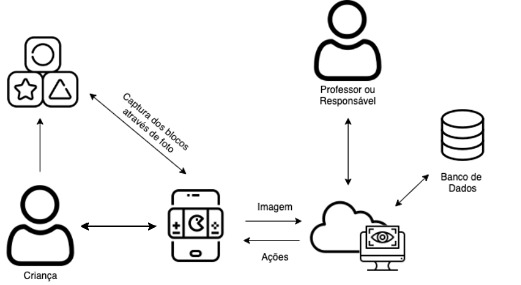
\includegraphics[width=\linewidth]{Imagens/Cap3/Visao_Geral.jpg}
        \legend{\small{Fonte: o autor (2020)}}
        \label{figura:visao_geral}
    \end{figure}
    
    \begin{figure}[H]
        \caption{Diagrama de blocos para submissão do desafio}
        \centering
        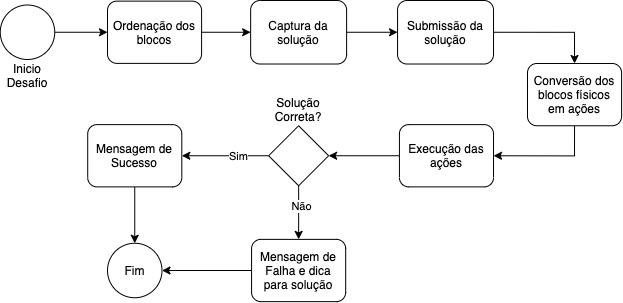
\includegraphics[width=\linewidth]{Imagens/Cap3/Blocos Desafio.jpg}
        \legend{\small{Fonte: o autor (2020)}}
        \label{figura:blocos_desafio}
    \end{figure}
    
    A análise da imagem será por meio de visão computacional a fim de identificar os blocos utilizados e convertê-los em ações. Ao final da conversão, o servidor salvará a solução submetida no banco de dados e retornará as ações para o jogo executar, representado no diagrama da Figura \ref{figura:blocos_reconhecimento}. O professor/tutor terá acesso a um link para visualizar todas as submissões das crianças, além de gráficos estatísticos comparando-as.
    
    \begin{figure}[H]
        \caption{Diagrama de blocos para reconhecimento dos blocos}
        \centering
        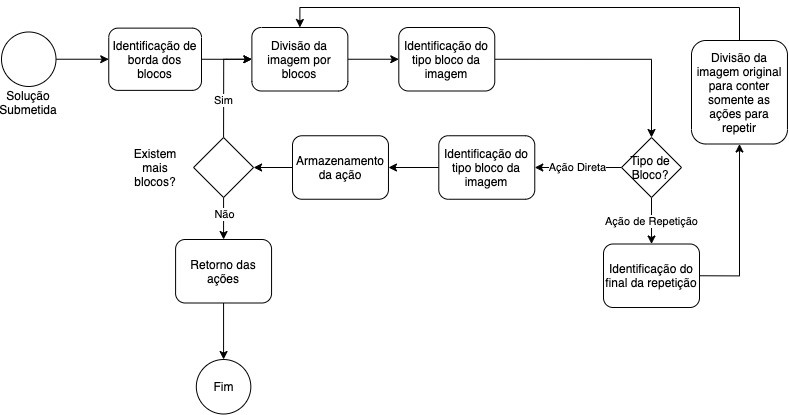
\includegraphics[width=\linewidth]{Imagens/Cap3/Blocos Reconhecimento.jpg}
        \legend{\small{Fonte: o autor (2020)}}
        \label{figura:blocos_reconhecimento}
    \end{figure}
    
    \subsection{Condições Restritivas}
    O projeto proposto apresenta algumas condições restritivas, conforme descrito nos próximos subitens.

        \subsubsection{Custos}
        Apesar do jogo precisar de materiais relativamente baratos para ser jogado, como blocos impressos em 3D ou até mesmo papéis coloridos dobrados de forma semelhante aos blocos impressos, ainda se faz necessário o uso de um celular com sistema operacional Android com câmera para que o aplicativo funcione. 
        % Escrever sobre custos de impressão dos blocos
            
        \subsubsection{Físicas e Ambientais}
        Apesar, quando impressos em 3D, dos bloco terem uma boa durabilidade, com o passar do tempo ficarão inutilizáveis. Portanto deve-se orientar os usuários do aplicativo jogo a fazer o descarte adequado dos blocos físicos depois de inutilizáveis, seja por desgaste dos blocos ou por falta de uso, o que vai de encontro com uma das propostas levantada pelo aplicativo jogo, a reciclagem.
        
        \subsubsection{Tecnológicas}
        O aplicativo jogo necessita de um celular com câmera e com o sistema operacional Android com a versão igual ou superior a 5.0 - Lollipop. Por se tratar de um protótipo, o aplicativo não oferece suporte para os demais dispositivos móveis com outros sistemas operacionais, como por exemplo iPhones. 
        
        \subsubsection{Energização}
        O dispositivo móvel é limitado em relação à energia, tendo um período máximo que uma carga pode sustentar, esse período máximo varia conforme o modelo e o uso do dispositivo. Para diminuir os efeitos causado por essa limitação, recomenda-se o uso do aplicativo com a bateria cheia ou próximo a uma tomada caso seja necessário recarregar a bateria do dispositivo móvel.    
        
        \subsubsection{Interferências devido ao meio}
        O aplicativo jogo precisa de conexão com internet para funcionar. Obstáculos como objetos metálicos ou paredes podem causar interferências no sinal Wi-Fi. Eletrônicos e eletrodomésticos, como por exemplo micro-ondas, operam na mesma frequência do roteador wireless, 2,4 GHz, que quando ligados, também podem contribuir com interferências dificultando ou até impossibilitando o uso do aplicativo.
        % Escrever sobre o posicionamento da camera e dos blocos
    
    \subsection{Benefícios e Impactos}
    O aplicativo jogo apresenta alguns benefícios e impactos, conforme descrito nos próximos subitens.

        \subsubsection{Econômicos}
        Além de um celular com câmera, o aplicativo jogo proposto é capaz de funcionar com recursos relativamente baratos, como blocos impressos em 3D ou até mesmo uma folha colorida dobrada em formatos semelhantes aos cubos; o aplicativo jogo também funciona de forma simples. Portanto pode ser utilizado em casa ou implantado em escolas de forma fácil e econômica para proporcionar à crianças um contato inicial com temas como lógica de programação e sustentabilidade, além de atender às novas demandas da BNCC para o ensino.
        
        \subsubsection{Operacionais}
        O aplicativo jogo pode ser aplicado em ambiente escolar. Por ser uma ferramenta que difere dos métodos tradicionais de ensino das escolas, pode ser uma experiência lúdica o que impacta diretamente na rotina das crianças.
        
        \subsubsection{Estratégicos}
        A mais nova atualização da Base Nacional Comum Curricular destina uma de suas dez competência à educação integral por meio de tecnologias digitais e faz uso, no caderno de matemática, do termo “pensamento computacional”. Pensando nisso, o aplicativo jogo proposto possibilita, de uma forma estratégica, um meio para trabalhar essas competências nas escolas. 
        
        \subsubsection{Políticos}
        Não se aplica.

        \subsubsection{Sociais}
        O aplicativo jogo apresenta benefícios sociais para as crianças, pois as crianças terão acessos a conceitos básicos de lógica de programação e oportunidade de exercitar esse conceitos, o que pode auxiliar em competências como raciocínio lógico, resolução de problemas, pensamento computacional, entre outras habilidades que tem sido cada vez mais requisitadas no mercado de trabalho. 
        Isso sendo proporcionado por um jogo, além de gerar maior engajamento no ensino de crianças, pode desenvolver, também, competências como cooperação, cumprimento de regras, controle de impulsividade, auxílio na tomada de decisões, mais facilidade para lidar com erros e fracassos entre outras habilidades sociais.
        Além disso, o aplicativo jogo, por meio do tema de reciclagem, pode desenvolver senso de sustentabilidade auxiliando na compreensão da importância do descarte correto do lixo, o que impacta direta e positivamente  o meio ambiente.
        % Revisar escrita

\section{Análise Funcional e de Requisitos Tecnológicos}
    Nessa sessão, é apresentada a análise funcional e os requisitos tecnológicos do sistema.

    \subsection{Lista de Funcionalidade e Atores}
    O sistema será composto  pelas seguintes funcionalidades:
    \begin{itemize}
        \item Desafios de lógica com o tema reciclagem;
        \item Identificação dos blocos;
        \item Conversão dos blocos em ações;
        \item Relatórios de jogo para acompanhamento do professor.
    \end{itemize}
    
    O sistema tem como atores a criança e o professor/tutor. A criança é responsável pela interação com os blocos e aplicativo.
    O professor/tutor é responsável pela interação com os dados adquiridos durante a partida da criança.
    
    \subsection{Comunicação}
    A comunicação entre o aplicativo e o servidor ocorrerá de maneira bidirecional e utilizará arquitetura \textit{REST}, através da conexão Wi-Fi com a Internet.
    O aplicativo envia os dados e imagens para o servidor. Após o servidor salvar os dados e processar as imagens, ele retorna as ações a serem executadas para o aplicativo.
    
    O \textit{REST (Representational State Transfer)} é uma abstração da arquitetura da \textit{Web}. Consistem em regras que permitem a criação de projetos com interfaces bem definidas, permitindo a comunicação entre aplicações.
    
    \subsection{Processamento}
    O processamento por parte do software, ocorre tanto no aplicativo quanto no servidor. O jogo captura as imagens e as envia para o servidor através da Internet. O servidor recebe as imagens enviadas pelo aplicativo e passa cada uma pelo algoritmo de visão computacional, responsável pela identificação de cada bloco nas fotos. Após a identificação dos blocos, é salvo a sequência no banco de dados e as ações são enviadas para o aplicativo.
    Após receber o retorno com as ações, o aplicativo transforma as ações em código e executa o mesmo durante o jogo.
    
    O jogo possuirá 4 desafios, cada um explorando um tipo de bloco. Ao inicio de cada fase, será executado uma animação para mostrar a ação que o tipo de bloco apresentado na fase executará juntamente com a sua forma de utilização.
    A primeira fase, apresentada na Figura \ref{figura:fase_1} trabalha a utilização do bloco andar. Para completar a fase com sucesso, a criança precisará utilizar uma combinação de três blocos andar para coletar o lixo e levá-lo a lixeira correta. Ao final dessa fase, será apresentado um vídeo informativo sobre o descarte correto de plástico.
    
    \begin{figure}[H]
        \caption{Fase 1}
        \centering
        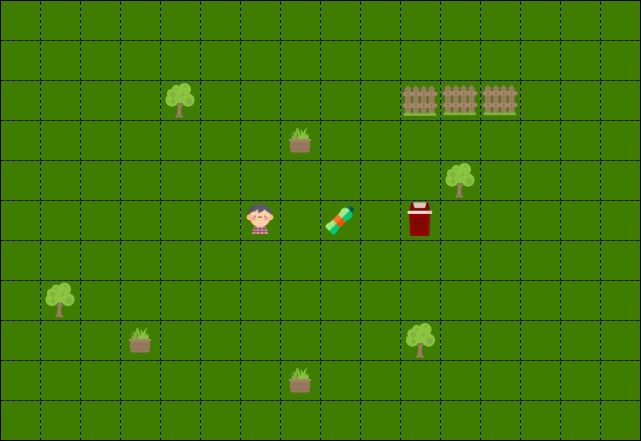
\includegraphics[width=12cm]{Imagens/Cap3/Fases/Fase1.jpg}
        \legend{\small{Fonte: o autor (2020)}}
        \label{figura:fase_1}
    \end{figure}
    
    A segunda fase, apresentada na Figura \ref{figura:fase_2} trabalha a utilização do bloco virar noventa graus. Para completar a fase com sucesso, a criança precisará utilizar uma combinação de quatro blocos andar e um bloco virar 90 graus para coletar o lixo e levá-lo a lixeira correta. Ao final dessa fase, será apresentado um vídeo informativo sobre o descarte correto de papel.
    
    \begin{figure}[H]
        \caption{Fase 2}
        \centering
        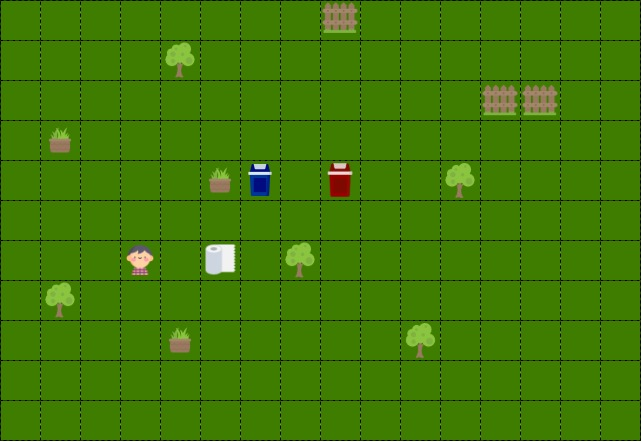
\includegraphics[width=12cm]{Imagens/Cap3/Fases/Fase2.jpg}
        \legend{\small{Fonte: o autor (2020)}}
        \label{figura:fase_2}
    \end{figure}
    
    A terceira fase, apresentada na Figura \ref{figura:fase_3} trabalha a utilização do bloco esperar. Para completar a fase com sucesso, a criança precisará utilizar uma combinação de cinco blocos andar e um bloco esperar para coletar o lixo e levá-lo a lixeira correta. Ao final dessa fase, será apresentado um vídeo informativo sobre o descarte correto de metal.
    
    \begin{figure}[H]
        \caption{Fase 3}
        \centering
        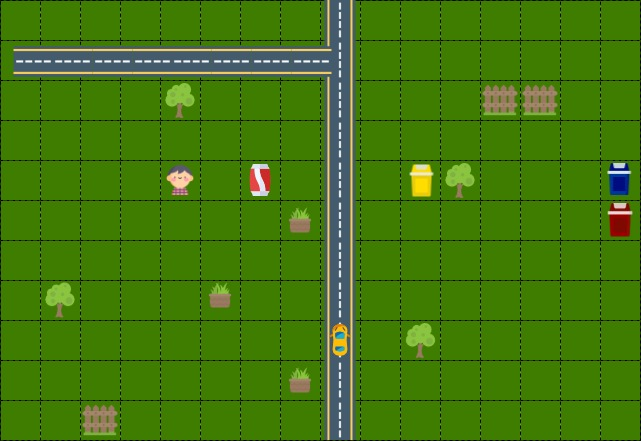
\includegraphics[width=12cm]{Imagens/Cap3/Fases/Fase3.jpg}
        \legend{\small{Fonte: o autor (2020)}}
        \label{figura:fase_3}
    \end{figure}
    
    A quarta fase, apresentada na Figura \ref{figura:fase_4} trabalha a utilização do bloco de repetição. Para completar a fase com sucesso, a criança precisará utilizar uma combinação de quatro blocos andar, um bloco esperar e um bloco virar 90 graus juntamente do bloco de repetição e o bloco numérico 2 para coletar o lixo e levá-lo a lixeira correta. Ao final dessa fase, será apresentado um vídeo informativo sobre o descarte correto de vidro.
    
    \begin{figure}[H]
        \caption{Fase 4}
        \centering
        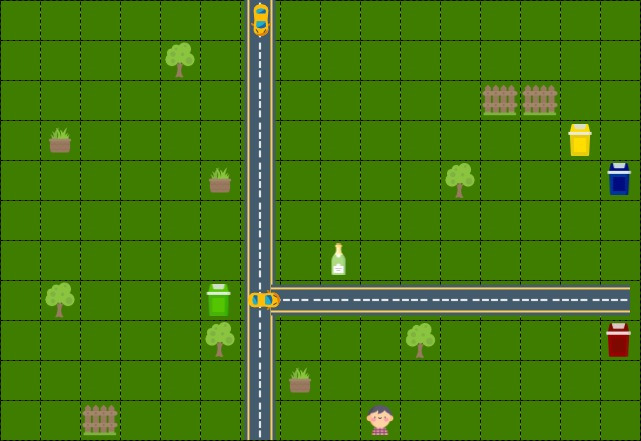
\includegraphics[width=12cm]{Imagens/Cap3/Fases/Fase4.jpg}
        \legend{\small{Fonte: o autor (2020)}}
        \label{figura:fase_4}
    \end{figure}
    
    % Escrever sobre o processamento das imagens.
    
    \subsection{Interface Homem-Máquina}
    As interações da criança serão com os blocos físicos e com o aplicativo.
    Na tela inicial, são apresentadas duas opções, créditos e desafios, como mostra a Figura \ref{figura:tela_inicial}.
    
    \begin{figure}[H]
        \caption{Tela Inicial}
        \centering
        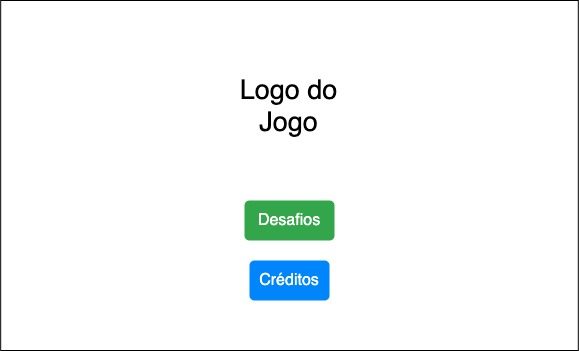
\includegraphics[width=\linewidth]{Imagens/Cap3/Tela Inicial.jpg}
        \legend{\small{Fonte: o autor (2020)}}
        \label{figura:tela_inicial}
    \end{figure}
    
    Ao acessar a opção de desafios é apresentada a lista de todos os desafios disponíveis, juntamente com o progresso de cada desafio (se disponível), conforme apresentado na Figura \ref{figura:tela_desafios}.
    
    \begin{figure}[H]
        \caption{Tela de Desafios}
        \centering
        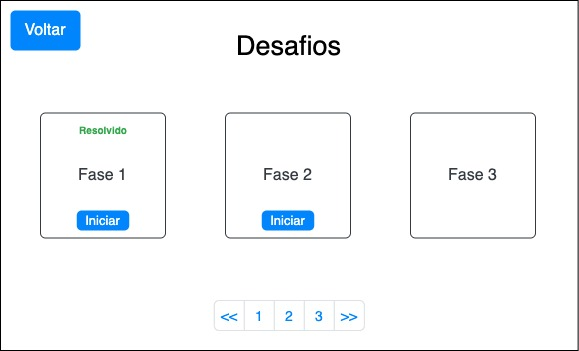
\includegraphics[width=\linewidth]{Imagens/Cap3/tela_desafios.jpg}
        \legend{\small{Fonte: o autor (2020)}}
        \label{figura:tela_desafios}
    \end{figure}
    
    Nessa tela, é possível ver a lista de desafios, um desafio só poderá ser iniciado caso o anterior tenha sido resolvido.
    É possível clicar no botão voltar para retornar à tela anterior. Ao clicar no botão iniciar do desafio, a criança poderá ser direcionada para a tela de cadastro ou direto para a tela do desafio. Caso a criança não tenha preenchido as informações para identificá-la, essas informações serão coletadas em uma tela específica, conforme Figura \ref{figura:cadastro}. Caso contrário ela é direcionada para a tela que contém o desafio a ser solucionado.
    
    \begin{figure}[H]
        \caption{Tela de Cadastro}
        \centering
        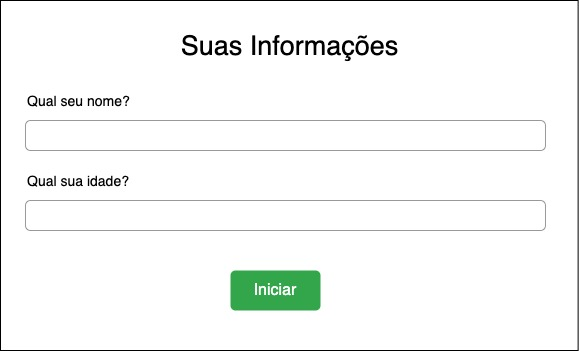
\includegraphics[width=\linewidth]{Imagens/Cap3/informacoes_usuario.jpg}
        \legend{\small{Fonte: o autor (2020)}}
        \label{figura:cadastro}
    \end{figure}
    
    A Figura \ref{figura:tela_jogo} mostra a interface principal durante o jogo.
    
    \begin{figure}[H]
        \caption{Tela do Jogo}
        \centering
        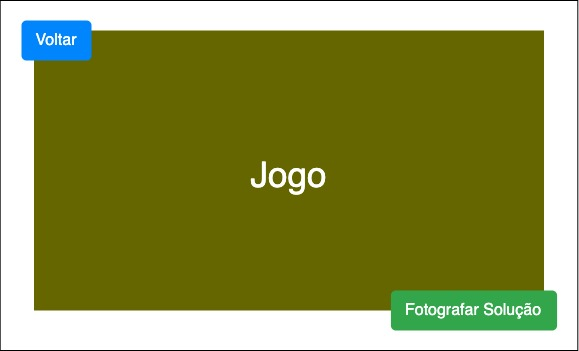
\includegraphics[width=\linewidth]{Imagens/Cap3/tela_jogo.jpg}
        \legend{\small{Fonte: o autor (2020)}}
        \label{figura:tela_jogo}
    \end{figure}
    
    Nessa tela é possível executar duas ações. Clicando no botão voltar, a criança é redirecionada para a lista de desafios. Selecionando o botão Fotografar Solução, é aberta uma janela, conforme Figura \ref{figura:fotografar_blocos} para fotografar a solução.
    
    \begin{figure}[H]
        \caption{Tela para fotografar a solução}
        \centering
        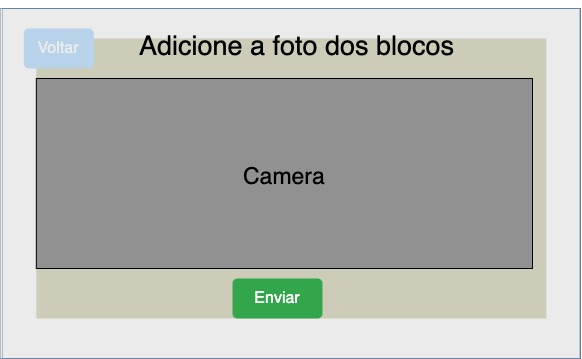
\includegraphics[width=\linewidth]{Imagens/Cap3/UploadSolucao.jpg}
        \legend{\small{Fonte: o autor (2020)}}
        \label{figura:fotografar_blocos}
    \end{figure}
    
    Cada bloco deve ser fotografado e adicionado utilizando o botão Novo Bloco.
    Ao fotografar todos os blocos, pode-se clicar no botão enviar para que a solução seja processada.
    Após a conversão da foto em ações para o jogo, o usuário é direcionado para a tela de jogo onde as ações convertidas serão executadas.
    Caso o personagem chegue com o lixo na lixeira correta , será apresentada uma mensagem de sucesso, conforme Figura \ref{figura:solucao_correta}. Caso contrário, será apresentada a mensagem de falha, permitindo uma nova tentativa, Figura \ref{figura:solucao_incorreta}.
    
    \begin{figure}[H]
        \caption{Mensagem de solução correta}
        \centering
        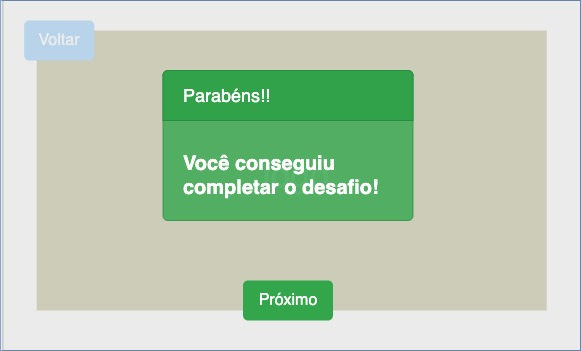
\includegraphics[width=\linewidth]{Imagens/Cap3/solucao_correta.jpg}
        \legend{\small{Fonte: o autor (2020)}}
        \label{figura:solucao_correta}
    \end{figure}
    
    \begin{figure}[H]
        \caption{Mensagem de solução incorreta}
        \centering
        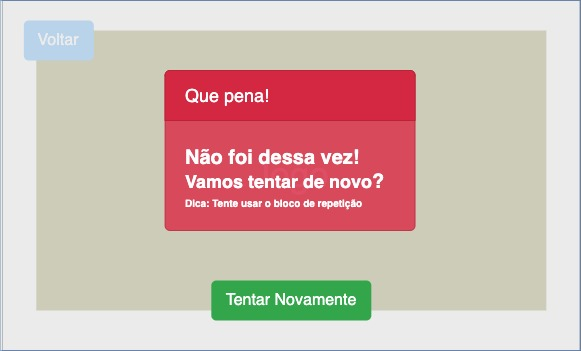
\includegraphics[width=\linewidth]{Imagens/Cap3/solucao_incorreta.jpg}
        \legend{\small{Fonte: o autor (2020)}}
        \label{figura:solucao_incorreta}
    \end{figure}
    
    O tutor terá acesso a um link para visualizar o relatório com as submissões das crianças conforme mostra a Figura \ref{figura:tela_relatorios}. Será possível ver todas as soluções enviadas além de relatórios estatísticos sobre o progresso no jogo.
    
    \begin{figure}[H]
        \caption{Tela de Relatórios}
        \centering
        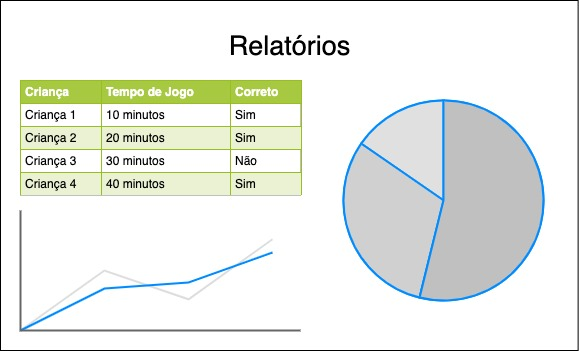
\includegraphics[width=\linewidth]{Imagens/Cap3/Tela Relatorios.jpg}
        \legend{\small{Fonte: o autor (2020)}}
        \label{figura:tela_relatorios}
    \end{figure}
    
    \subsection{Sistemas Controlados Automaticamente}
    O Sistema não apresentará sistemas controlados automaticamente.
    
    \subsection{Aquisição de dados e Atuação}
    A coleta das fotos se dará através da ação da criança que está jogando. Após concluir a proposta de solução do desafio, a criança deve capturar sua proposta utilizando a câmera do dispositivo móvel, como mostrado na Figura \ref{figura:crianca_blocos}.
    
    \begin{figure}[H]
        \caption{Criança capturando a solução}
        \centering
        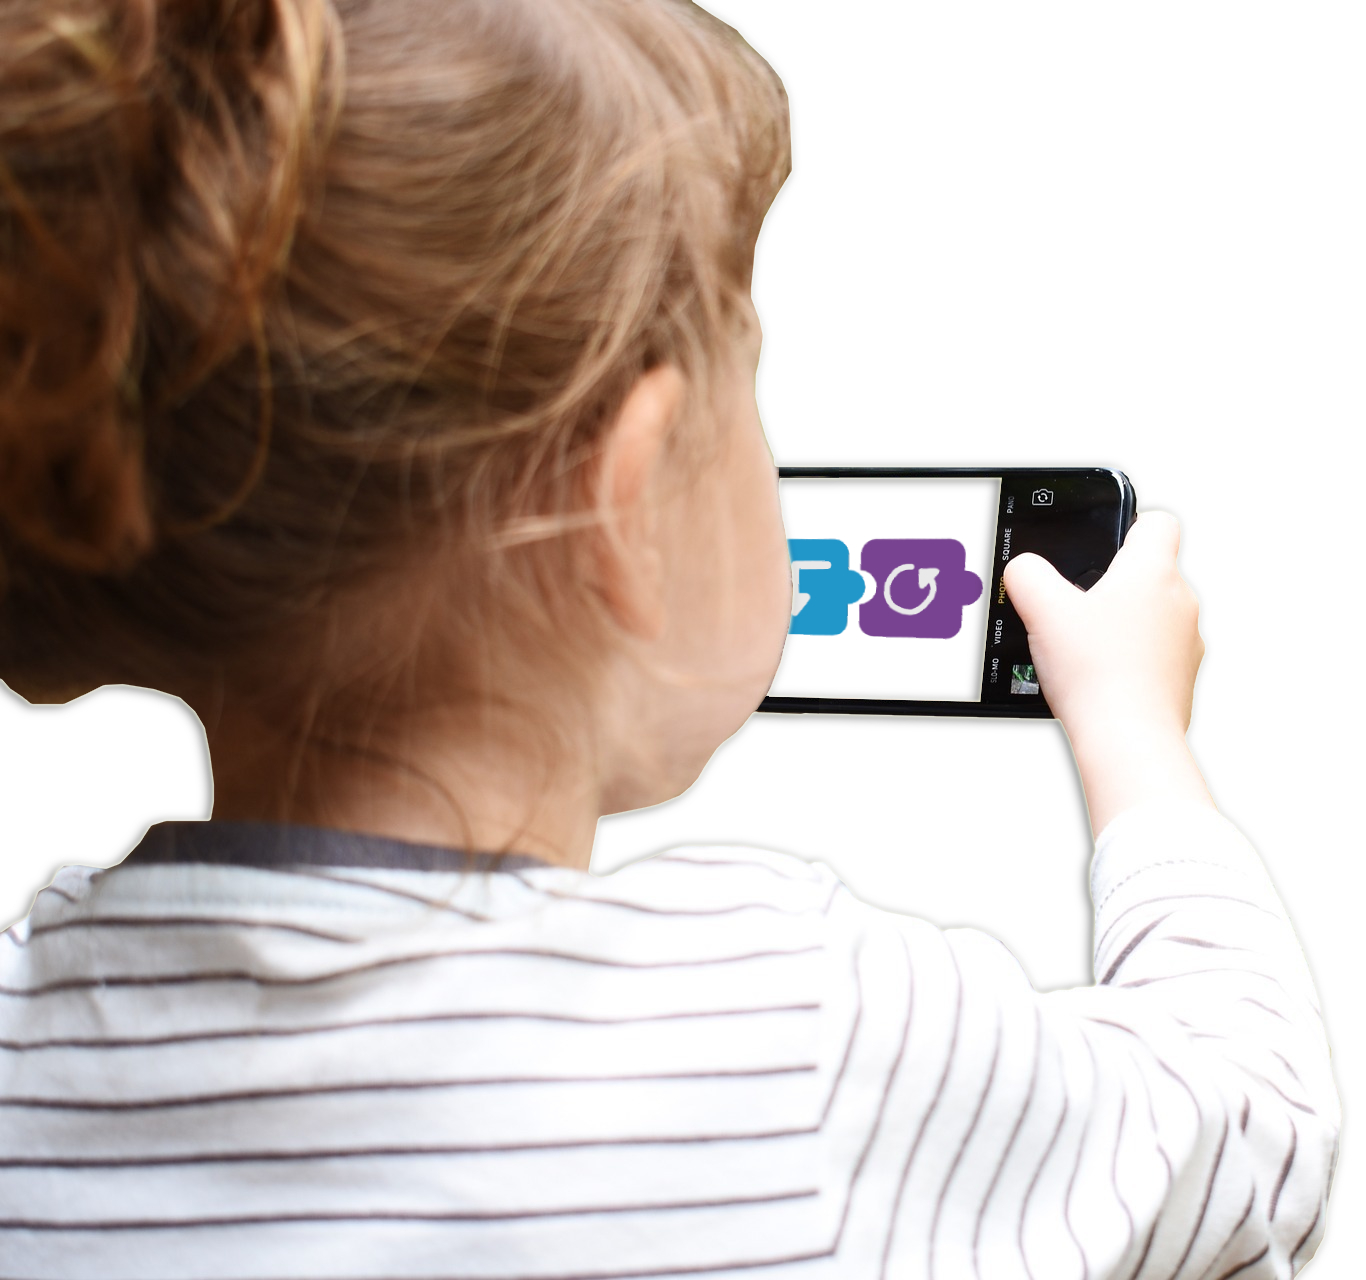
\includegraphics[width=10cm]{Imagens/Cap3/CriançaBlocos.jpg}
        \legend{\small{Fonte: o autor (2020)}}
        \label{figura:crianca_blocos}
    \end{figure}
    
    Após a captura da imagem, a criança, utilizando um botão de envio, submeterá a foto para o servidor.
    
    O envio da foto e o recebimento da conversão em ações do jogo é realizado através de conexão com a Internet.
    Toda proposta de solução, esteja ela correta ou não, será salva no banco de dados, após sua interpretação, para gerar relatórios estatísticos.


\section{Análise da Arquitetura do Sistema}
    Nessa sessão, são apresentadas as arquiteturas de hardware e software do sistema.

    \subsection{Hardware}
    O hardware do sistema será composto por blocos físicos e o dispositivo mobile com câmera. O dispositivo mobile deverá ser um celular \textit{Android} com câmera, podendo variar entre os modelos existentes no mercado.
    
    Os blocos físicos serão construídos de PLA, impressos em 3D, com o tamanho aproximado de 10cm x 10cm x 5mm, seus cantos serão arredondados para evitar acidentes no manuseio. Para facilitar a identificação, cada bloco possuirá uma cor especifica juntamente com um símbolo representando a sua ação.
    Os blocos são dividos em duas categorias, sendo elas, ações e blocos numéricos. As ações são divididas em dois tipos, ações diretas e repetição. A Figura \ref{figura:blocos_fisicos} apresenta todos os blocos disponíveis no protótipo.
    
    \begin{figure}[H]
        \caption{Blocos Físicos}
        \centering
        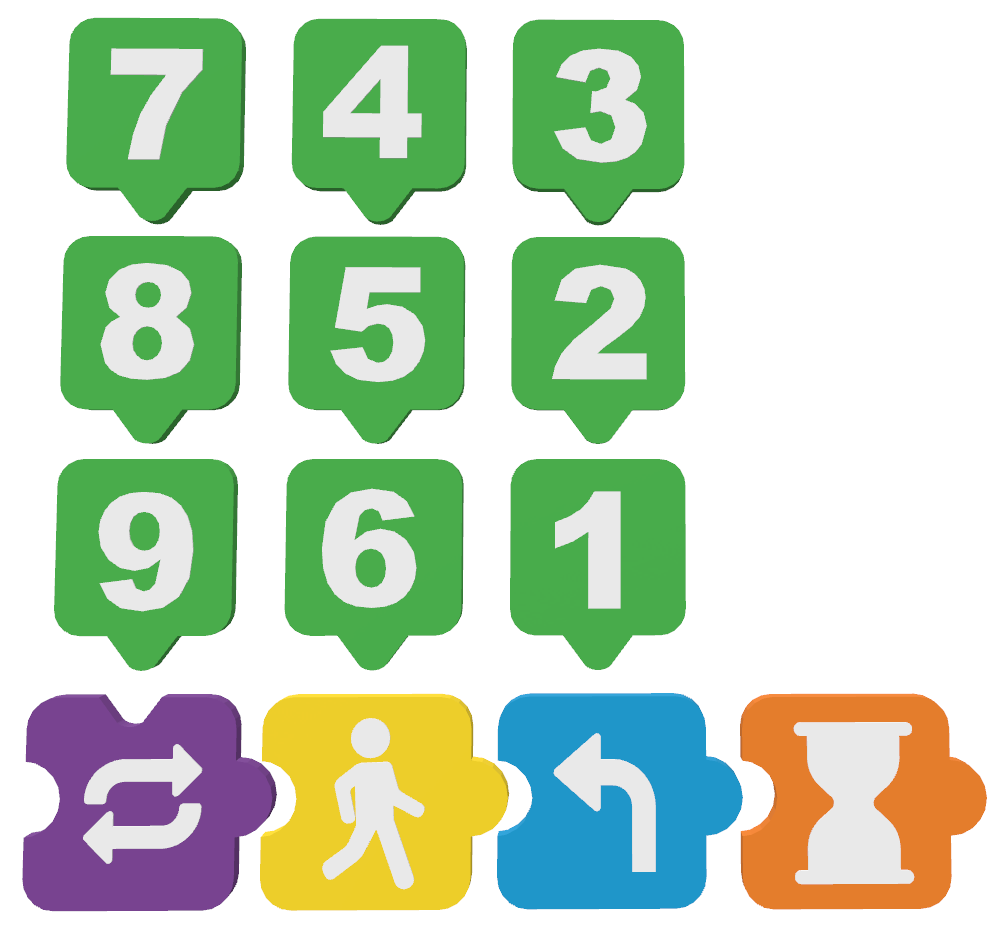
\includegraphics[width=\linewidth]{Imagens/Cap3/Blocos/Todos.png}
        \legend{\small{Fonte: o autor (2020)}}
        \label{figura:blocos_fisicos}
    \end{figure}
    
    \subsubsection{Blocos Numéricos}
        Os blocos numéricos são identificados pela cor verde e pelos números de um a nove, conforme apresentado na Figura \ref{figura:blocos_numericos}. Eles possuem um encaixe diferente dos demais, somente encaixam nos blocos de repetição, pois são utilizados para identificar a quantidade de vezes que o bloco de repetição irá repetir. Não podem ser utilizados com outros blocos ou até mesmo sozinho.
        
        \begin{figure}[H]
            \caption{Blocos Numéricos}
            \centering
            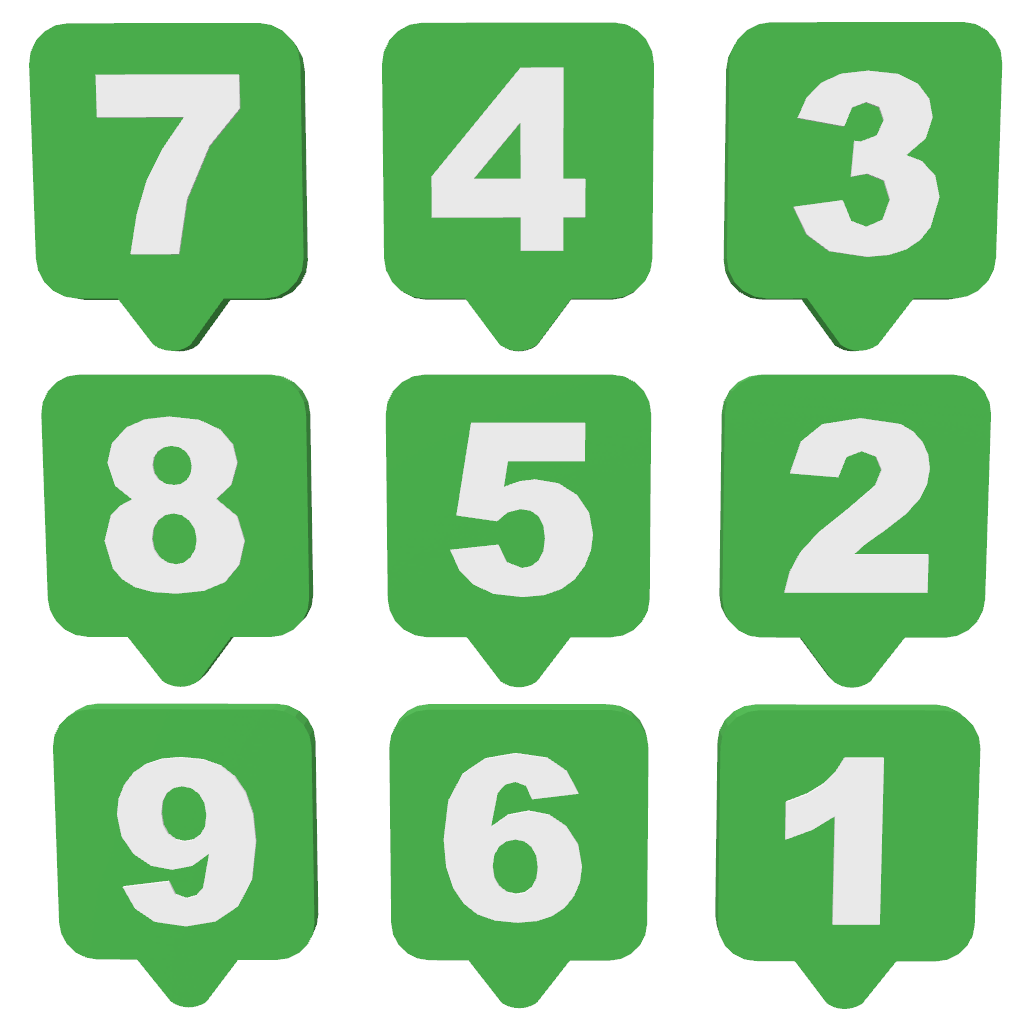
\includegraphics[width=10cm]{Imagens/Cap3/Blocos/Blocos_Numericos.png}
            \legend{\small{Fonte: o autor (2020)}}
            \label{figura:blocos_numericos}
        \end{figure}
    
    \subsubsection{Ações Diretas}
        As ações diretas são ações que não possuem necessidade de outros blocos, ou seja, podem ser utilizadas sozinhas.
        O jogo possui 3 ações diretas, sendo elas, andar, virar noventa graus e esperar. 
        A ação andar movimenta o personagem para frente uma única vez, seu bloco é identificado pela cor amarela e pelo simbolo de um boneco andando, conforme apresentado na Figura \ref{figura:andar}.
        
        \begin{figure}[H]
            \caption{Andar}
            \centering
            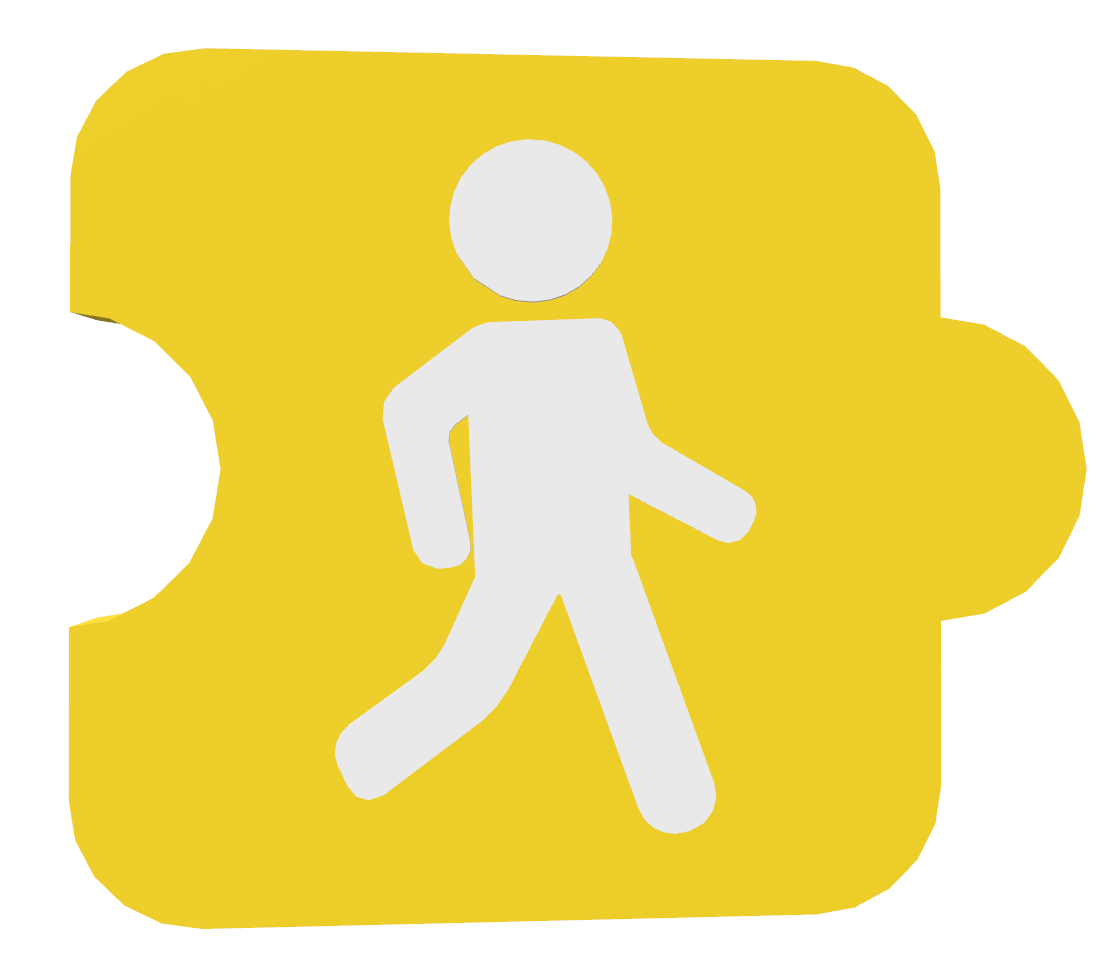
\includegraphics[width=5cm]{Imagens/Cap3/Blocos/Andar.png}
            \legend{\small{Fonte: o autor (2020)}}
            \label{figura:andar}
        \end{figure}
        
        A ação virar noventa graus rotaciona o personagem noventa graus para a esquerda, seu bloco é identificado pela cor azul e o simbolo de uma seta apontando para a esquerda, conforme apresentado na Fugira \ref{figura:virar}.
        
        \begin{figure}[H]
            \caption{Virar noventa graus}
            \centering
            
\includegraphics[width=5cm]{Imagens/Cap3/Blocos/Virar.png}
            \legend{\small{Fonte: o autor (2020)}}
            \label{figura:virar}
        \end{figure}
        
        A ação esperar mantém o personagem parado no cenário, sem executar nenhuma outra ação, seu bloco é identificado pela cor laranja e o simbolo de uma ampulheta, conforme apresentado na Figura \ref{figura:esperar}
        
        \begin{figure}[H]
            \caption{Esperar}
            \centering
            
\includegraphics[width=5cm]{Imagens/Cap3/Blocos/Esperar.png}
            \legend{\small{Fonte: o autor (2020)}}
            \label{figura:esperar}
        \end{figure}
        
    \subsubsection{Ação de Repetição}
        A ação de repetição é identificada pela cor roxa e pelo simbolo de duas flechas em formato oval, conforme apresentado na Figura \ref{figura:repetir}. É uma ação que possui necessidade de mais blocos para ser executada, não podendo ser utilizada sozinha.
        
        \begin{figure}[H]
            \caption{Repetir}
            \centering
            
\includegraphics[width=5cm]{Imagens/Cap3/Blocos/Repetir.png}
            \legend{\small{Fonte: o autor (2020)}}
            \label{figura:repetir}
        \end{figure}
        
        Para criar uma repetição é preciso a utilização de um bloco de repetição seguido das ações diretas a serem repetidas e outro bloco de repetição para finalização. Possui um encaixe na parte superior para ser colocado um bloco numérico, que identificará a quantidade de vezes que as ações devem ser executadas. O bloco numérico precisará constar somente no bloco de repetição de inicio. Caso não seja utilizado um bloco numérico em conjunto, ficará executando infinitamente. A Figura \ref{figura:exemplo_repeticao} mostra um exemplo de repetição, onde as ações andar e virar noventa graus serão repetidas infinitamente.
        
        \begin{figure}[H]
            \caption{Exemplo de repetição}
            \centering
            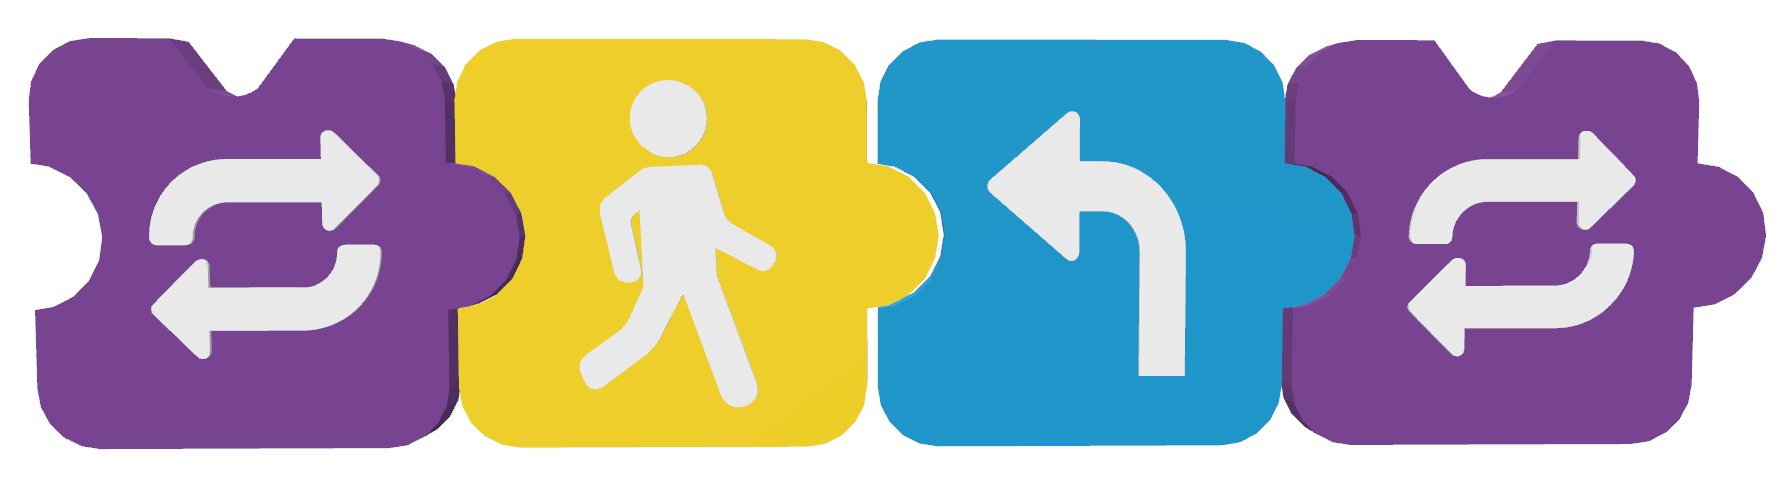
\includegraphics[width=\linewidth]{Imagens/Cap3/Blocos/Exemplo_Repeticao.png}
            \legend{\small{Fonte: o autor (2020)}}
            \label{figura:exemplo_repeticao}
        \end{figure}
    
    \subsection{Software}
    O jogo será desenvolvido para celulares Android utilizando o Unity 3D. A arquitetura do software para reconhecimento dos blocos será baseada em serviços cloud, utilizando a IBM Cloud como provedor.
    O servidor, programado em Python, utilizará o serviço IBM Cloud Foundry. O banco de dados, não relacional, utilizará o serviço IBM Cloudant.
    
    O Cloud Foundry é um servico \textit{PAAS (Platform as a Service)} que permite implementar e ajustar a escala de aplicativos de maneira rápida, simples e barata. O IBM Cloudant é um serviço de banco de dados distribuído, desenvolvido no Apache CouchDB, é otimizado para grandes cargas e rápido crescimento.
    
    Nos tópicos a seguir, são apresentados os diagramas do software que representam o seu funcionamento.
        
        \subsubsection{Use Case}
        O jogo conta com funções de identificação da criança (perfil), inicio de desafio e submissão de solução, conforme apresentado no diagrama de caso de uso da criança na Figura \ref{figura:use_case}. A função de submissão de solução do jogo conversa diretamente com a função de reconhecimento dos blocos no servidor.
        O servidor conta com funções de relatórios e reconhecimento dos blocos. Apenas o professor/tutor poderá acessar os relatórios conforme apresentado no diagrama de caso de uso do tutor na Figura \ref{figura:use_case}.
        
        \begin{figure}[H]
            \caption{Caso de uso}
            \centering
                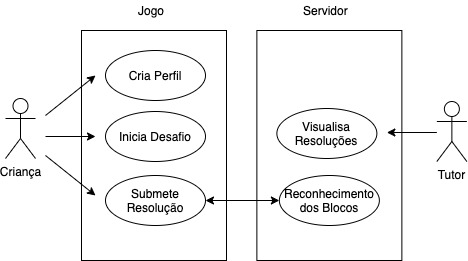
\includegraphics[width=15cm]{Imagens/Cap3/Use_Case.jpg}
            \legend{\small{Fonte: o autor (2020)}}
            \label{figura:use_case}
        \end{figure}
        
        \subsubsection{Diagramas de Sequência}
        
        Nesse tópico são apresentados os diagramas de sequencia para as funcionalidades principais do aplicativo.
        
        \subsubsubsection{Criação de Perfil}
        
        A Figura \ref{figura:sequencia_perfil} mostra o diagrama de sequência para a realização do cadastro de informações da criança. Todas as informações são salvas localmente para que, na submissão da solução, seja salvo um único objeto. 
        
        \begin{figure}[H]
            \caption{Diagrama de Sequência - Perfil}
            \centering
                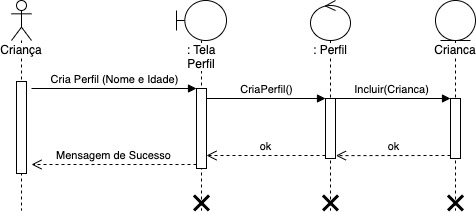
\includegraphics[width=\linewidth]{Imagens/Cap3/Sequencia_Perfil.jpg}
    
            \legend{\small{Fonte: o autor (2020)}}
            \label{figura:sequencia_perfil}
        \end{figure}
        
        \subsubsubsection{Submissão da Resolução}
        
        O diagrama apresentado na Figura \ref{figura:sequencia_jogo} mostra o processo de submissão da solução e validação da mesma.
        
        \begin{figure}[H]
            \caption{Diagrama de Sequência - Submissão da Resolução}
            \centering
                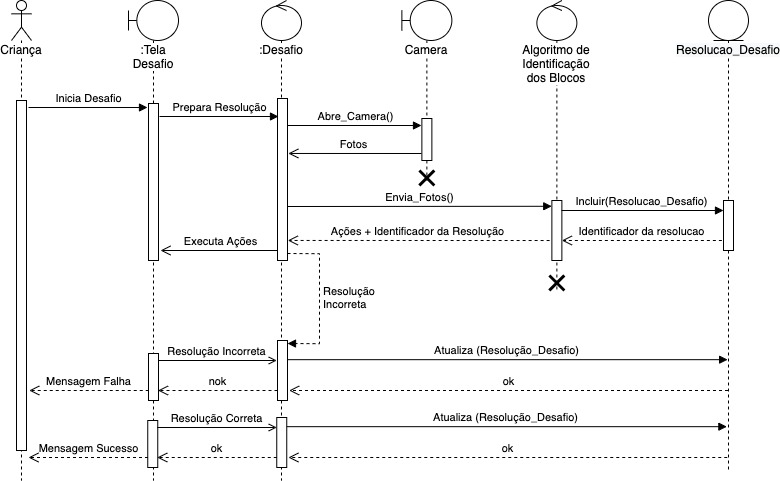
\includegraphics[width=\linewidth]{Imagens/Cap3/Sequencia_Jogo.jpg}
    
            \legend{\small{Fonte: o autor (2020)}}
            \label{figura:sequencia_jogo}
        \end{figure}
        
        Ao iniciar o desafio, a data e hora são salvos localmente para que, quando a resolução for submetida, essa informação seja salva junto com as demais no banco de dados. Após o aplicativo processar as ações convertidas pelo algoritmo de identificação dos blocos, o aplicativo valida a solução e atualiza a resolução no banco com o seu status, correto ou não correto.
        
        \subsubsubsection{Visualização de Relatório}
        
        O diagrama apresentado na Figura \ref{figura:sequencia_tutor} mostra o processo para o tutor visualizar os relatórios dos desafios submetidos pelas crianças.
        
        \begin{figure}[H]
            \caption{Diagrama de Sequência - Visualização de Relatório}
            \centering
                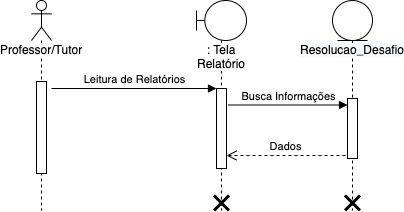
\includegraphics[width=\linewidth]{Imagens/Cap3/sequencia_tutor.jpg}
            \legend{\small{Fonte: o autor (2020)}}
            \label{figura:sequencia_tutor}
        \end{figure}
        
        O tutor receberá um link via e-mail para acessar o relatório das soluções submetidas pelas crianças. Ao acessar o link, a tela acessa o banco de dados para buscar as informações para popular os relatórios.